% Model-specific consequences of classical association and truncated moments.
\section{Additional Resource-Action and Probe-Value Plots}
Fig.~\ref{fig:joint-actions} retains the complete action plot for the joint-controller study in the main paper.
Fig.~\ref{fig:risk-reduction} retains its controlled probe-value comparisons; no data, caption or graphical content has changed.
\begin{figure}[t]
\centering
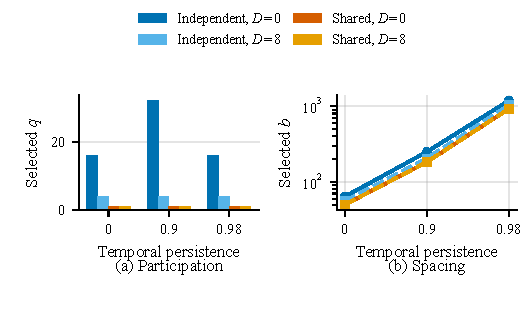
\includegraphics[width=\columnwidth]{figures/exp010b_joint_actions.pdf}
\caption{Joint actions selected by the finite-time Lyapunov certificate.
The left panel reports participation and the right panel reports Markov spacing; persistence values occupy categorical positions.}
\label{fig:joint-actions}
\end{figure}
\begin{figure}[t]
\centering
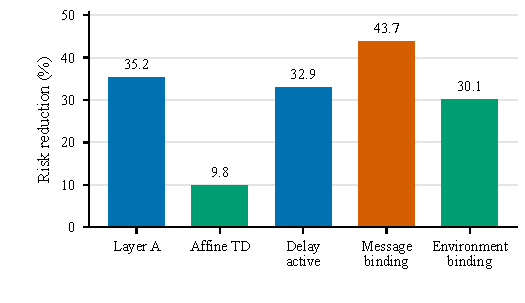
\includegraphics[width=\columnwidth]{figures/exp016b_risk_reduction.pdf}
\caption{Relative risk reductions of the learning-aware rule over information-only probing.
All percentages use information-only risk as the denominator.}
\label{fig:risk-reduction}
\end{figure}
\subsection{Retained confidence-stress and reproducibility details}
The Markov temporal-difference task has seven states on a ring, a bounded sinusoidal reward, four stationary-distribution-orthonormal features, and an exact projected fixed point.
Cross-agent dependence is induced by shared and private Markov sources while preserving every agent's marginal transition law.
The policy-learning studies use MAPPO with parameter-shared actors and a centralized critic~\maincite{yu2022mappo}.
They cover PettingZoo's multi-agent particle environment \texttt{simple\_spread\_v2}~\maincite{terry2021pettingzoo} and the multi-agent MuJoCo (MaMuJoCo) \texttt{HalfCheetah-v2/2x3} benchmark~\maincite{peng2021facmac}.
Bootstrap comparisons resample paired seeds and report percentile intervals for the ratio of geometric-mean risks.
The confidence-interface study uses 64 disjoint confirmation seeds and 157,440 checkpoint rows.
The moderate stress inflates $K_q$ and $\Omega_q$ by 10 percent and weakens the certified mixing log-rate by 0.05; the strong stress uses 25 percent and 0.10.
Both shields retain the nominal action in all twelve cells, all 24 stress-by-cell one-sided 99 percent upper means remain below the robust certificate, and neither shield changes empirical terminal risk.
Controlled statistics/curves reproduce byte for byte; robustness uses eight development and 64 disjoint confirmation seeds.
Each policy-learning study has 80 finite, exactly budgeted runs spanning both regimes and all policies; all 160 runs reproduce aggregate curves byte for byte.
These ablations quantify the terminal parameter-risk gain from the finite-horizon objective; the joint-action study isolates the response to correlation, spacing, and delay.
\section{Signed Continuing-Stream Risk and Fixed-Program Separation}
\label{sec:signed-mechanism}
The design-utility formulation is classical~\maincite{chaloner1995bayesian}; selection dependence and perfect-information value are also established objects~\maincite{russo2016bias}.
Here these tools are specialized to the paid, continuing-stream learner in main Eq.~\eqref{eq:linear-program}.
The distinctions below are the sign of its actual-risk transfer, explicit one-sided constants, and a full-budget comparator, not new general association, truncation, or decision-theory principles.

\subsection{Exact signed transfer for a fixed likelihood decision}
Freeze $a_0,a_1$, their remaining-budget horizons, and all weights before a deterministic probe.
Its vector $Y$ has laws $\mathcal N(0,\Sigma_j)$, where $0\prec\Sigma_0\preceq\Sigma_1$.
Use a fixed likelihood threshold and a fixed data-independent tie rule, selecting one for the outside event $Y^\top(\Sigma_0^{-1}-\Sigma_1^{-1})Y>c$.
Let $E_j$ be the wrong-decision event, $p_j=\Pr_j(E_j)$, $\Delta J_j=J_{j,a_{1-j}}-J_{j,a_j}$, and $\Delta_k=k_{a_1}^2-k_{a_0}^2$.
The coefficient $k_a$ is common to the hypotheses, as their persistence parameter is the same.
Write $\mathcal C_j=\E_j[(m_j^2-s_j^2)\mathbf1_{E_j}]$.
Symmetry and association give
\begin{align}
R_0&=J_{0,a_0}+p_0\Delta J_0+\Delta_k\mathcal C_0,\\
R_1&=J_{1,a_1}+p_1\Delta J_1-\Delta_k\mathcal C_1,\\
\mathcal C_0&\ge0,\quad\mathcal C_1\le0.
\label{eq:supp-signed-transfer}
\end{align}
To see this, subtract Eq.~\eqref{eq:supp-conditional-risk} for the wrong and correct programs.
The decision event is even in $Y$, whereas $m_j$ is linear and odd, so $\E_j[m_j\mathbf1_{E_j}]=0$, including nonzero deterministic initialization.
Whiten $Y$ under each true instance and orthogonally diagonalize the positive semidefinite decision quadratic.
The resulting coordinates $G_i$ are independent standard normal variables and the outside event is increasing in each $G_i^2$.
Writing $m_j=\sum_i v_iG_i$, coordinate sign symmetry eliminates all cross products.
Each diagonal covariance $\operatorname{Cov}(G_i^2,\mathbf1_{\rm outside})$ is nonnegative by association of independent variables~\maincite{esary1967association}, Theorem~2.1.
For completeness, condition on the other squares and use $2\operatorname{Cov}(f(X),g(X))=\E[(f(X)-f(X'))(g(X)-g(X'))]\ge0$ for increasing $f,g$ and an independent copy $X'$.
The inside event is the complement, which proves the other sign.
Thus $\Delta_k>0$ permits harmful carryover, $\Delta_k<0$ permits beneficial carryover, and $\Delta_k=0$ removes it exactly; strictness needs a nonconstant event and an aligned posterior component.
In the implemented model $\Sigma_j=I+Q\theta_jR_\lambda$, covariance ordering follows from $\theta_1>\theta_0$.

\subsection{Classical tail moments and a learner-specific corollary}
Let $\varphi$ and $\Phi$ be the standard normal density and distribution function.
For $0<p<1$, define
\begin{align*}
t_p&=\Phi^{-1}(1-p/2),& h_+(p)&=2t_p\varphi(t_p),\\
u_p&=\Phi^{-1}((1+p)/2),& h_-(p)&=2u_p\varphi(u_p).
\end{align*}
Set both $h_\pm(0)=0$ by continuity.
The truncated-normal moment calculation is classical~\maincite{manjunath2021moments}, Sections~2--3 and~5.
For any event $E$ of probability $p$ and $m\sim\mathcal N(0,s^2)$,
\begin{equation}
-s^2h_-(p)\le\E[(m^2-s^2)\mathbf1_E]\le s^2h_+(p).
\label{eq:supp-tail-moments}
\end{equation}
This also allows $E$ to depend on other variables.
Indeed, condition its indicator on $m$ to obtain an acceptance function $g(m)\in[0,1]$ of Gaussian mass $p$.
With $f(m)=m^2-s^2$, let $g_*$ select the tails $|m|>st_p$ and $c=s^2(t_p^2-1)$.
Then $(f-c)(g_*-g)\ge0$ pointwise, and the equal-mass constraint gives $\E[fg_*]\ge\E[fg]$.
Selecting the central interval $|m|\le su_p$ proves the minimum in the same way.
Integration by parts gives $\int_t^\infty(x^2-1)\varphi(x)\,dx=t\varphi(t)$, establishing Eq.~\eqref{eq:supp-tail-moments} and its sharp scalar constants.

\begin{proposition}[Ordered-Gaussian continuing-risk corollary]
Under the fixed-program, fixed-probe and centered ordered-covariance conditions above, suppose $p_j\le\delta_j\le1/4$.
Then
\begin{align}
R_0&\le J_{0,a_0}+\delta_0[\Delta J_0]_+
+[\Delta_k]_+s_0^2h_+(\delta_0),\\
R_1&\le J_{1,a_1}+\delta_1[\Delta J_1]_+
+[\Delta_k]_+s_1^2h_-(\delta_1).
\label{eq:supp-signed-upper}
\end{align}
\label{prop:supp-signed-risk}
\end{proposition}
\begin{proof}
On $[0,1/4]$, $h_+'(p)=t_p^2-1\ge0$ and $h_-'(p)=1-u_p^2\ge0$.
Combine Eq.~\eqref{eq:supp-signed-transfer} with Eq.~\eqref{eq:supp-tail-moments} and $p_j\Delta J_j\le\delta_j[\Delta J_j]_+$.
When $\Delta_k\le0$, the transfer term is nonpositive under both instances and can be omitted from an upper bound.
\end{proof}
For small $\delta$, $h_+(\delta)=O(\delta\log(1/\delta))$ and $h_-(\delta)=O(\delta)$.
The sharpness is for the scalar event-moment problem, not every finite probe geometry.
Data-dependent probe stopping, noncentered likelihoods, sign-sensitive classifiers, and data-selected program weights require a different analysis; main Theorem~\ref{thm:same-stream} remains available at its stated scope.

\subsection{Why independent-mixture transport can be insufficient}
Let $G,W$ be independent standard normals, $Y=\sqrt3(\rho G+\sqrt{1-\rho^2}W)$, and choose between the frozen programs $Z_0=1$ and $Z_1=(1+Y)/2$ using $E=\{|G|>t\}$.
Both unconditional squared risks equal one, yet
\begin{equation}
\E Z_{\rm selected}^2=1+\frac34\rho^2\,2t\varphi(t)>1
\label{eq:supp-mixture-counterexample}
\end{equation}
for $\rho\ne0$ and $0<t<\infty$.
Conditioning on $G$ gives $\E[Z_1^2\mid G]=1+(\sqrt3/2)\rho G+(3/4)\rho^2(G^2-1)$; the odd term cancels and Eq.~\eqref{eq:supp-tail-moments} evaluates the rest.
At $t=3$ and $\rho=1/2$, the event probability is $0.002699796$ and the risk is $1.004985829$.
An independent mixture incorrectly gives one even with the exact decision probability, because its unconditional branch-risk gap is zero.
This establishes the need to account for selection dependence in this linear Gaussian class, not necessity of a positive penalty when its signed transfer is beneficial.
It is an analytical example outside the registered family grid, not a counterexample to both tests of the executed AND-admission rule or a claim about cost-optimal branch choices.

\subsection{Classical decision comparison with paid continuing learners}
Fix the public family, learner, step rule and full budget, and let $\mathcal A_{\rm fix}$ contain all original full-budget fixed $(q,b)$ programs.
For a stated prior $\pi\in(0,1)$, define
\begin{align*}
I_\pi&=\min_{a\in\mathcal A_{\rm fix}}\{(1-\pi)J_0(a)+\pi J_1(a)\},\\
O_\pi&=(1-\pi)\min_aJ_0(a)+\pi\min_aJ_1(a),\\
V_\pi&=I_\pi-O_\pi.
\end{align*}
This is the finite-action value-of-perfect-information comparison already used in~\maincite{russo2016bias}, Section~2.6, with loss rather than utility.
The finite catalogue gives $V_\pi>0$ exactly when the two risk functions have no common minimizer: each fixed action's excess over $O_\pi$ is a positively weighted sum of two nonnegative excess risks, and the minimum is attained.
If $B_j$ is a valid actual-risk upper bound for the executed policy, main Eq.~\eqref{eq:fixed-catalogue-separation} proves lower prior-weighted risk than every fixed catalogue action, including every regime-independent randomized mixture by linearity.
To expose the cost balance, let $L_j=J_{j,a_j}^{\rm post}-\min_aJ_j(a)$ and $D_j=B_j-J_{j,a_j}^{\rm post}$.
The same sufficient condition is
\begin{equation}
V_\pi>(1-\pi)(L_0+D_0)+\pi(L_1+D_1).
\label{eq:supp-paid-opportunity}
\end{equation}
Here $L_j$ can be signed unless risk monotonicity in horizon has separately been proved for the affine transient.
Thus decision opportunity must exceed remaining-horizon and decision-event risk, not merely produce an accurate classification.
The reference $O_\pi$ allows a regime-informed fixed commitment, not arbitrary state-adaptive programs; $V_\pi=0$ does not exclude useful same-stream state selection.
The comparison fixes the learner, step rule and catalogue and is prior-specific, rather than a statement about all fixed algorithms, unknown priors or minimax risk.

\subsection{Complete original-design diagnostic}
This outcome-known deterministic calculation retains all 128 original designs and introduces no trajectory, seed or confidence interval.
The catalogues contain 16 actions at $Q=8$ and 24 at $Q=32$, including all original spacings and full-budget affordable horizons.
Of 120 feasible probes, 44 have potentially harmful transfer, 32 beneficial transfer and 44 zero transfer; eight infeasible designs remain included.
The original and sign-refined admission counts are both 113/128.
All 44 harmful designs were already admitted under the original enclosure, and removing the penalty does not rescue the seven feasible rejections.
These deterministic decisions explain the unchanged no-carryover ablation without attributing its equality to seed noise.

\begin{table}[t]
\centering
\caption{Full original-grid, balanced-prior population certificates using the executed gate's original bound, not a newly executed policy.}
\label{tab:supp-fixed-catalogue}
\begin{tabular}{lrr}
\toprule
Budget scale & Running mean & Delayed affine\\
\midrule
32 & 0/16 & 0/16\\
128 & 0/16 & 0/16\\
512 & 6/16 & 2/16\\
2048 & 12/16 & 9/16\\
\bottomrule
\end{tabular}
\end{table}
For $\pi=1/2$, 72/128 designs have positive $V_\pi$, while the original gate's bound certifies separation in 29/128, as shown in Table~\ref{tab:supp-fixed-catalogue}.
Their relative certified margins range from $0.1314$ to $7.2032$ percent of $I_{1/2}$; this range is not an average empirical effect.
All 99 uncertified balanced cases remain; zero of 128 satisfy the separate sufficient minimax comparison $\max_jB_j<\min_a\max_jJ_j(a)$.
These population-model diagnostics explain conditional usefulness and do not replace the validation's prespecified regime-stratified endpoints.
The original adverse low-budget result, 23/256 adverse cell means, identical corrected/no-carryover trajectories, and fixed $(2,1)$ pooled risk advantage all remain unchanged.
